\documentclass{article}

\usepackage[english]{babel}
\usepackage[utf8]{inputenc}
\usepackage{amsmath}
\usepackage{amsthm}
\usepackage{amssymb}
\usepackage{mathtools}
\usepackage{amsfonts}
\usepackage{subcaption}
\usepackage{graphicx}
\usepackage{wrapfig}
\usepackage{bbm}
\usepackage{dsfont}
\usepackage{listings}

% set up margin
\usepackage
[
  a4paper,
  left=3cm,
  right=3cm,
  top=3cm,
  bottom=3cm,
]
{geometry}

% set up header
\usepackage{fancyhdr}
\pagestyle{fancy}
\fancyhf{}
\lhead{6.438 Algorithms for Inference}
\chead{Problem Set 4}
\rhead{Hongzi Mao}
\cfoot{\thepage}
\rfoot{\footnotesize{\emph{Collaborated with: Hongzhou Ye, Zhiwei Ding}}}

% footer line
\renewcommand{\footrulewidth}{0.4pt}

% sans serif italic
\newcommand{\s}[1]{\textsf{\textit{#1}}}

% bold face sans serif
\newcommand{\bs}[1]{\textsf{\textbf{#1}}}

% set symbol
\usepackage[mathscr]{euscript}

% empty set
\let\emptyset\varnothing

% qed
\newcommand{\qeds}{\hfill\qedsymbol}

% math bold face
\newcommand{\bm}{\mathbf}

% argmax
\DeclareMathOperator*{\argmax}{argmax}
\DeclareMathOperator*{\argmin}{argmin}

% independence symbol
\makeatletter
\newcommand*{\indep}{%
  \mathbin{%
    \mathpalette{\@indep}{}%
  }%
}
\newcommand*{\nindep}{%
  \mathbin{%                   % The final symbol is a binary math operator
    \mathpalette{\@indep}{\not}% \mathpalette helps for the adaptation
                               % of the symbol to the different math styles.
  }%
}
\newcommand*{\@indep}[2]{%
  \sbox0{$#1\perp\m@th$}%        box 0 contains \perp symbol
  \sbox2{$#1=$}%                 box 2 for the height of =
  \sbox4{$#1\vcenter{}$}%        box 4 for the height of the math axis
  \rlap{\copy0}%                 first \perp
  \dimen@=\dimexpr\ht2-\ht4-.2pt\relax
  \kern\dimen@
  {#2}
  \kern\dimen@
  \copy0 %                       second \perp
} 
\makeatother

%%%%%%%%%%%%%%%%%%%%%%%%%%%%%%%%%%%%%%%%%%%%%%%%%%%%%%%%%%%%%%%%%%%%%%%%
%%%%%%%%%%%%%%%%%%%%%%%%% Begin document here %%%%%%%%%%%%%%%%%%%%%%%%%%
%%%%%%%%%%%%%%%%%%%%%%%%%%%%%%%%%%%%%%%%%%%%%%%%%%%%%%%%%%%%%%%%%%%%%%%%
\begin{document}

\section*{Problem 4.1}
%
(a) The desired function $f(\cdot)$ has the form
\begin{align*}
	f(\hat{x}_i) = 1 - \hat{x}_i.
\end{align*}
\\

\noindent
(b)
%
Consider the following arrangements of $p_{\s{x}_1, \s{x}_2}(\cdot, \cdot)$
and $p'_{\s{x}_1, \s{x}_2}(\cdot, \cdot)$,
\begin{align*}
	p_{\s{x}_1, \s{x}_2}(1, 1) &= 1/10,\\
	p_{\s{x}_1, \s{x}_2}(0, 1) &= 2/10,\\
	p_{\s{x}_1, \s{x}_2}(0, 0) &= 3/10,\\
	p_{\s{x}_1, \s{x}_2}(1, 0) &= 4/10,
\end{align*}

and
\begin{align*}
	p'_{\s{x}_1, \s{x}_2}(1, 1) &= 2/10,\\
	p'_{\s{x}_1, \s{x}_2}(0, 1) &= 1/10,\\
	p'_{\s{x}_1, \s{x}_2}(0, 0) &= 4/10,\\
	p'_{\s{x}_1, \s{x}_2}(1, 0) &= 3/10.
\end{align*}

Then the marginals coincide, since
\begin{align*}
	p_{\s{x}_1}(1) = p_{\s{x}_1, \s{x}_2}(1, 0) + p_{\s{x}_1, \s{x}_2}(1, 1) = 4/10 + 1/10 = 1/2,\\
	p'_{\s{x}_1}(1) = p'_{\s{x}_1, \s{x}_2}(1, 0) + p'_{\s{x}_1, \s{x}_2}(1, 1) = 3/10 + 2/10 = 1/2,
\end{align*}

and
\begin{align*}
	p_{\s{x}_2}(1) = p_{\s{x}_1, \s{x}_2}(0, 1) + p_{\s{x}_1, \s{x}_2}(1, 1) = 2/10 + 1/10 = 3/10,\\
	p'_{\s{x}_2}(1) = p'_{\s{x}_1, \s{x}_2}(0, 1) + p'_{\s{x}_1, \s{x}_2}(1, 1) = 1/10 + 2/10 = 3/10.
\end{align*}

But the desired states for $p_{\s{x}_1, \s{x}_2}(\cdot, \cdot)$
and $p'_{\s{x}_1, \s{x}_2}(\cdot, \cdot)$ are different, since
\begin{align*}
	\argmin_{x_1, x_2}\ p_{\s{x}_1, \s{x}_2}(1-x_1, 1-x_2) = (0, 0),\\
	\argmin_{x_1, x_2}\ p'_{\s{x}_1, \s{x}_2}(1-x_1, 1-x_2) = (1, 0).
\end{align*}\qeds
\\

\noindent
(c)
%
Consider the following arrangement for $p_{\s{x}_1, \s{x}_2}(\cdot, \cdot)$,
\begin{align*}
	p_{\s{x}_1, \s{x}_2}(1, 1) &= 4/10,\\
	p_{\s{x}_1, \s{x}_2}(0, 1) &= 1/10,\\
	p_{\s{x}_1, \s{x}_2}(0, 0) &= 2/10,\\
	p_{\s{x}_1, \s{x}_2}(1, 0) &= 3/10.
\end{align*}

Now the MAP estimates differ from the desired states, since
\begin{align*}
	&\argmax_{x_1, x_2}\ p_{\s{x}_1, \s{x}_2}(x_1, x_2) = (1, 1),\\
	&\argmin_{x_1, x_2}\ p_{\s{x}_1, \s{x}_2}(1-x_1, 1-x_2) = (1, 0).
\end{align*}\qeds
\\

\noindent
(d)
%
Notice that the potential are all positive, we can replace each potential with its reciprocal, i.e., let edge potential $\psi^{\text{new}}_{i, j}(\cdot, \cdot) = 1/\psi_{i, j}(\cdot, \cdot)$ for all edges in HMM.
Now in Viterbi algorithm, at each step of the max-product in the new graph, the argmax will correspond
to the argmin for the original graph. At the end, we can flip the arguments (i.e., take $1-x_i$ for each $i$)
to obtain the desired states.

\pagebreak
%%%%%%%%%%%%%%%%%%%%%%%%%%%%%%%%%%%%%%%%%%%%%%%%%%%%%%%%%%%%%%%%%%%%%%%% 
\section*{Problem 4.3}
(a)
%
Triangulating graph (a) with red edges:
\begin{figure}[h]
  \centering
  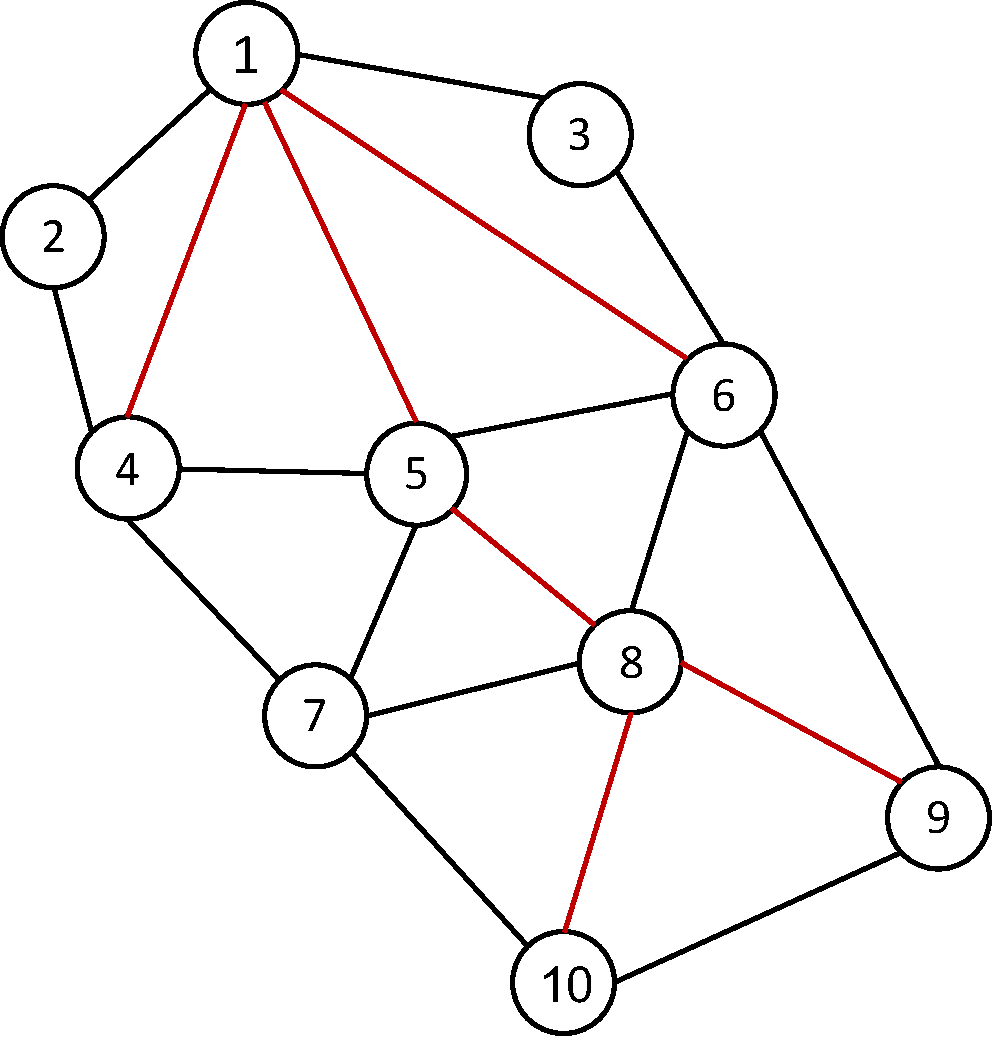
\includegraphics[width=0.25\columnwidth]{3a1.pdf}
    \vspace{-0.1cm}
\end{figure}

Applying greedy algorithm to construct the junction tree, with edge weights at each step
\begin{figure}[h]
  \centering
  \begin{subfigure}[b]{0.315\textwidth}
  	\centering
  	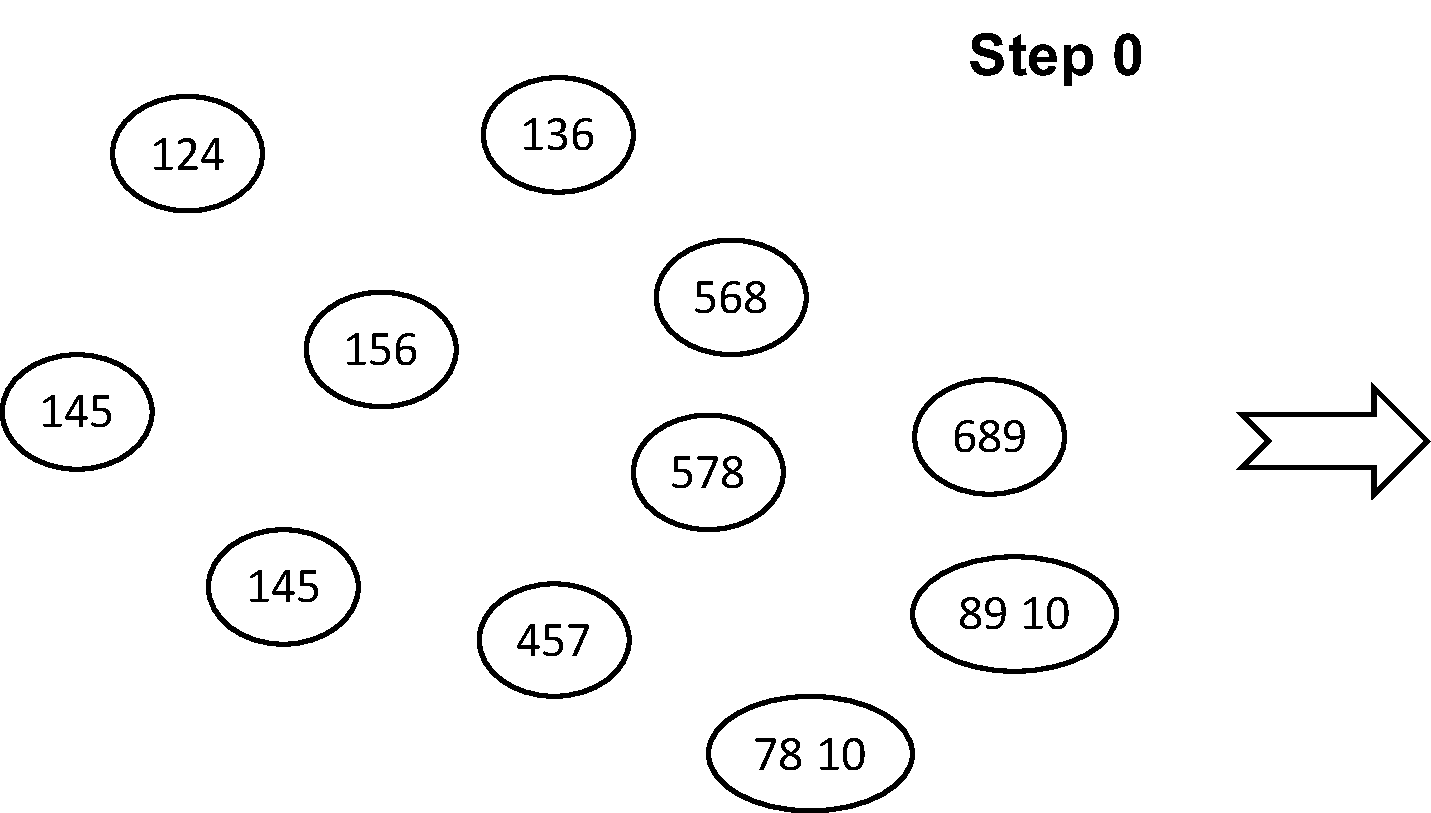
\includegraphics[width=\columnwidth]{3a2.pdf}
  \end{subfigure}
  \hspace{0.1cm}
  \begin{subfigure}[b]{0.315\textwidth}
    \centering
  	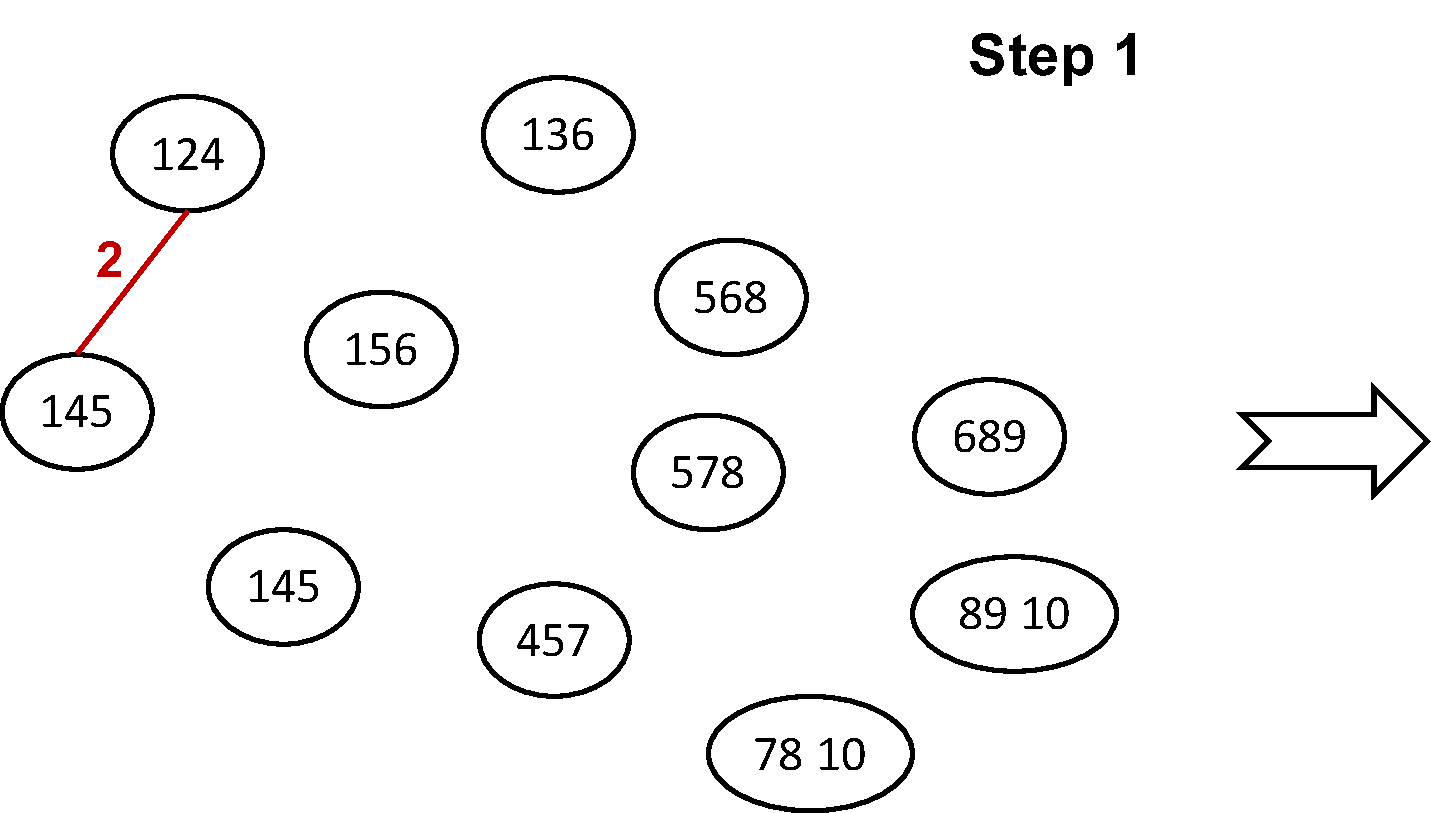
\includegraphics[width=\columnwidth]{3a3.pdf}
  \end{subfigure}
  \hspace{0.1cm}
  \begin{subfigure}[b]{0.315\textwidth}
    \centering
  	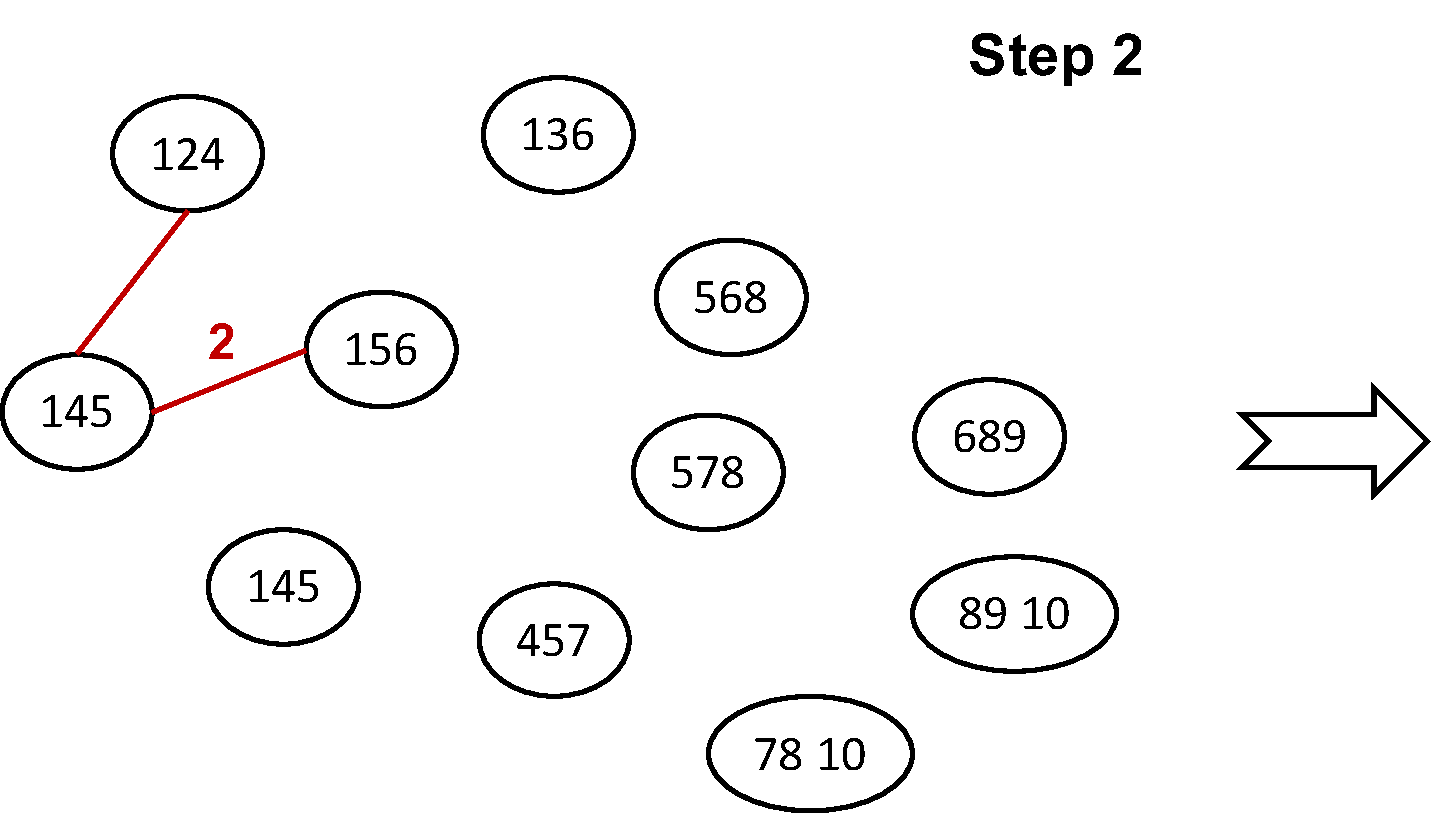
\includegraphics[width=\columnwidth]{3a4.pdf}
  \end{subfigure}
  \hspace{0.1cm}
    \begin{subfigure}[b]{0.315\textwidth}
  	\centering
  	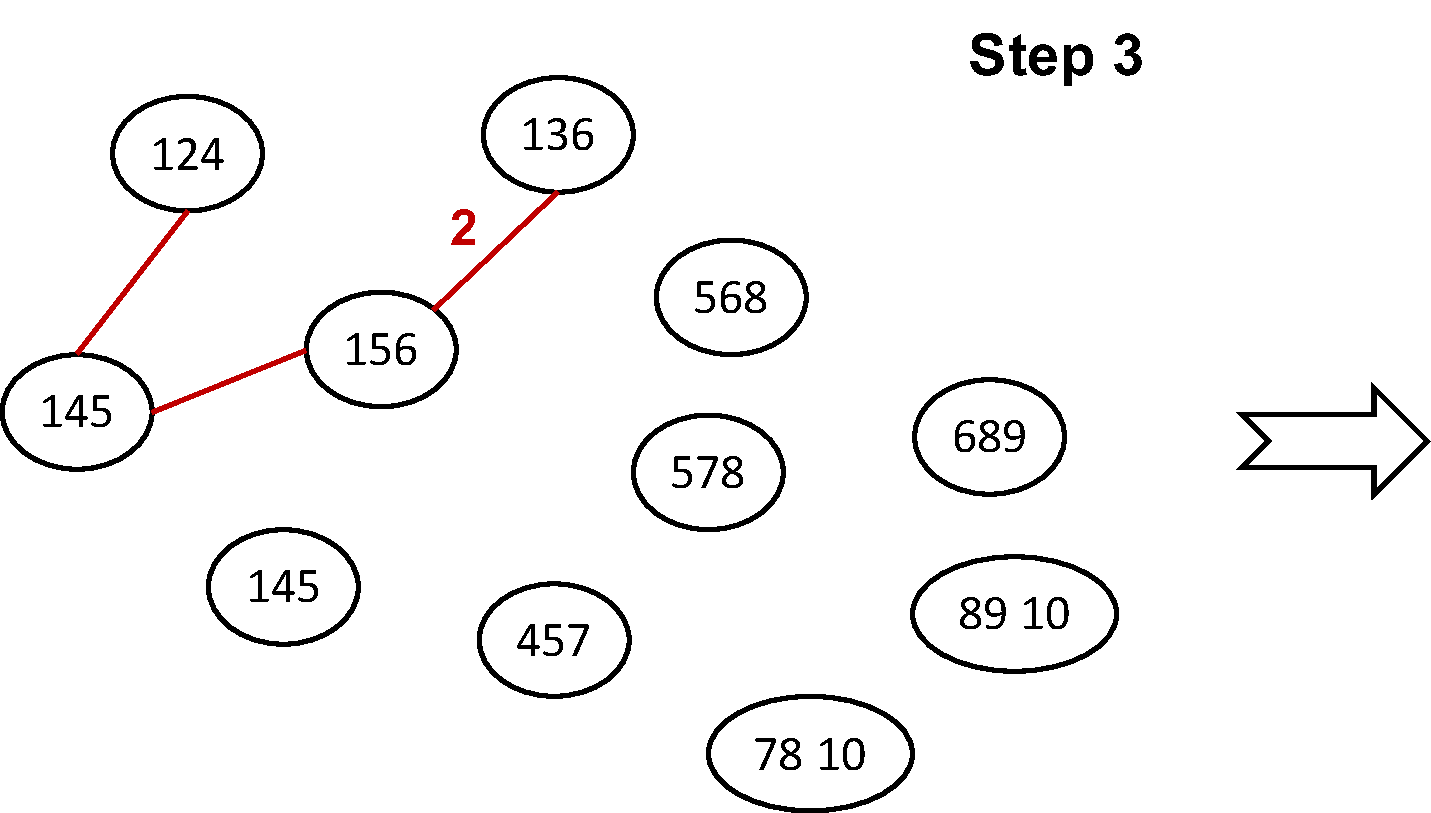
\includegraphics[width=\columnwidth]{3a5.pdf}
  \end{subfigure}
  \hspace{0.1cm}
  \begin{subfigure}[b]{0.315\textwidth}
    \centering
  	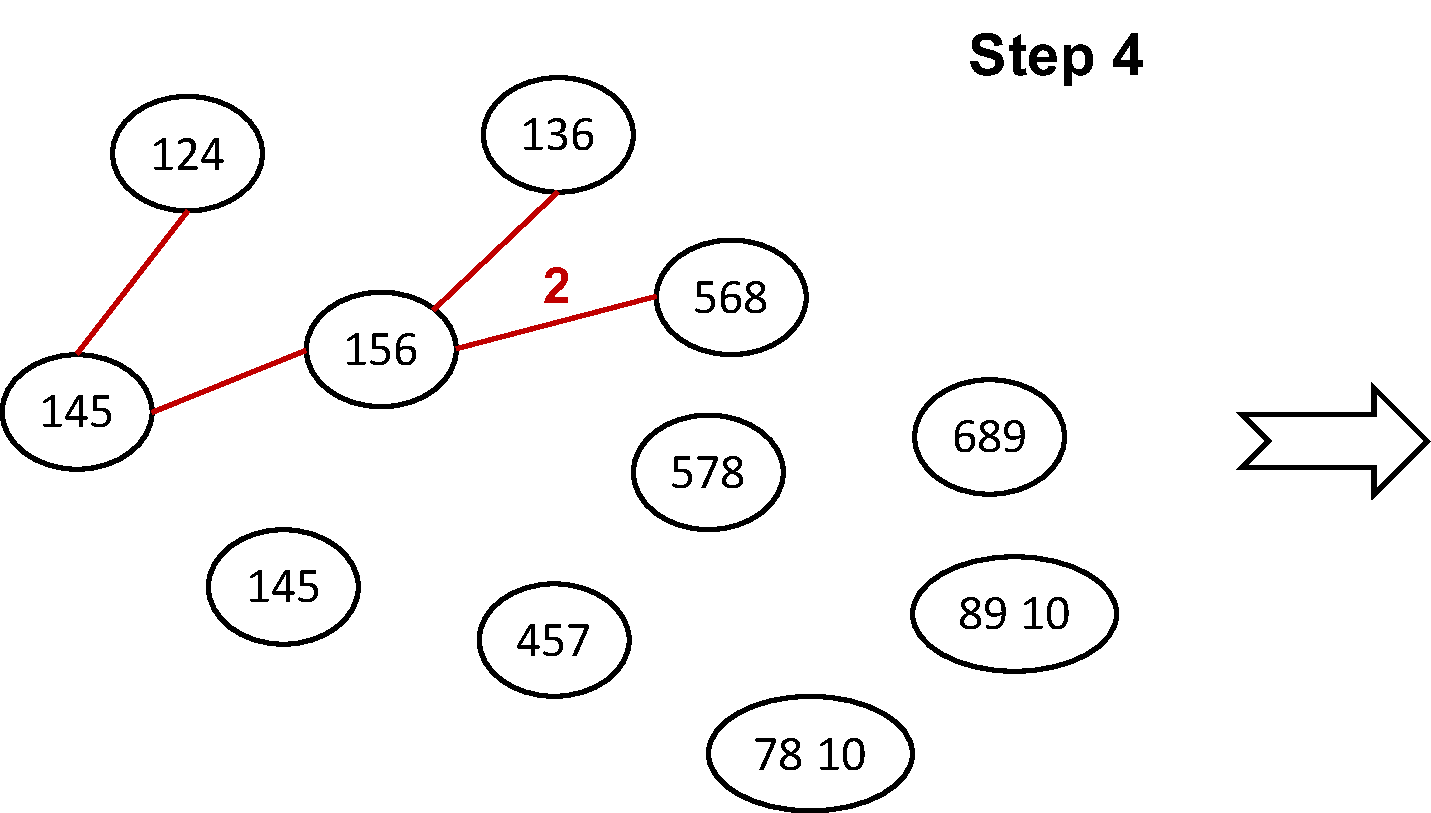
\includegraphics[width=\columnwidth]{3a6.pdf}
  \end{subfigure}
  \hspace{0.1cm}
  \begin{subfigure}[b]{0.315\textwidth}
    \centering
  	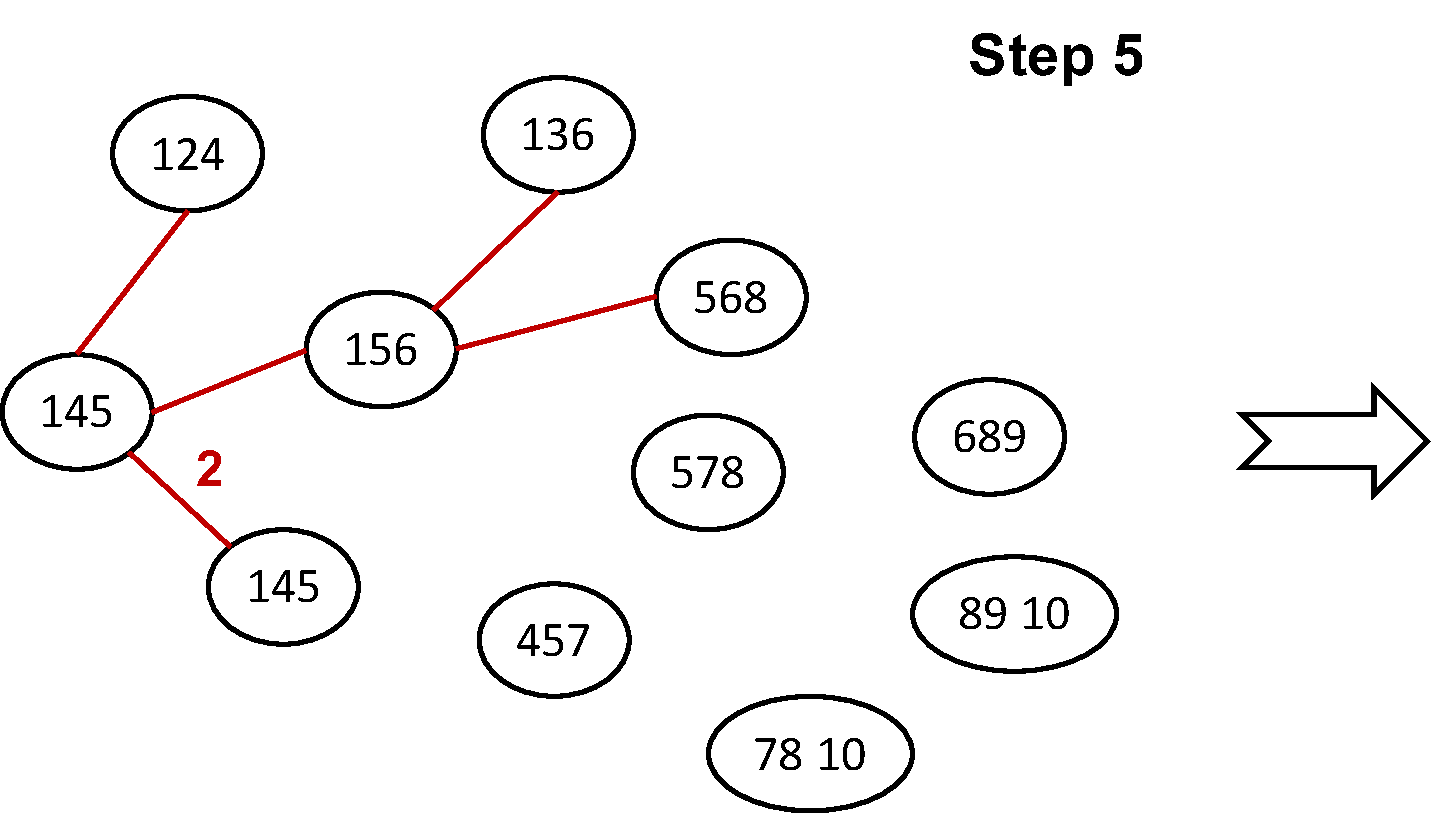
\includegraphics[width=\columnwidth]{3a7.pdf}
  \end{subfigure}
  \hspace{0.1cm}
    \begin{subfigure}[b]{0.315\textwidth}
  	\centering
  	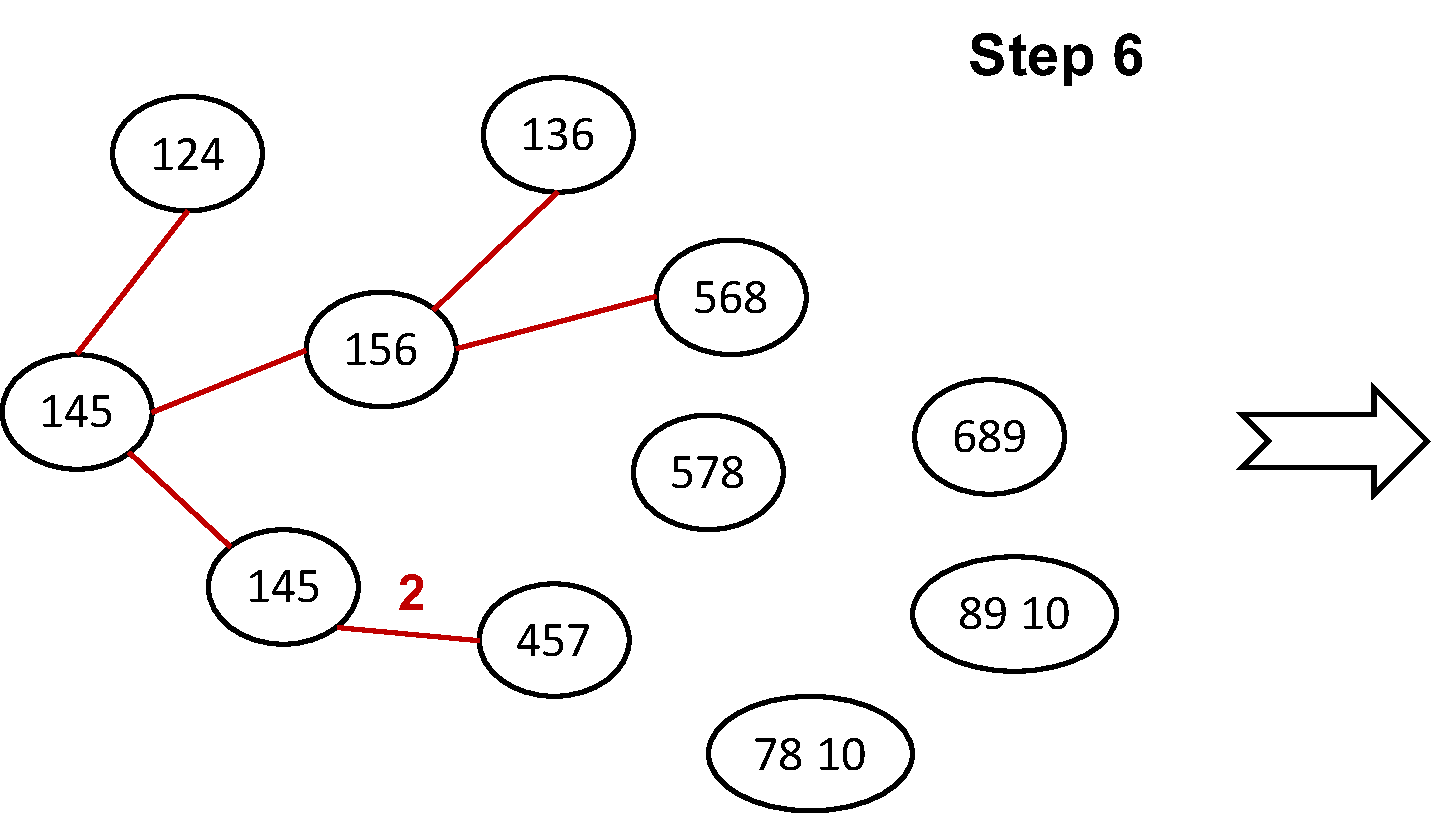
\includegraphics[width=\columnwidth]{3a8.pdf}
  \end{subfigure}
  \hspace{0.1cm}
  \begin{subfigure}[b]{0.315\textwidth}
    \centering
  	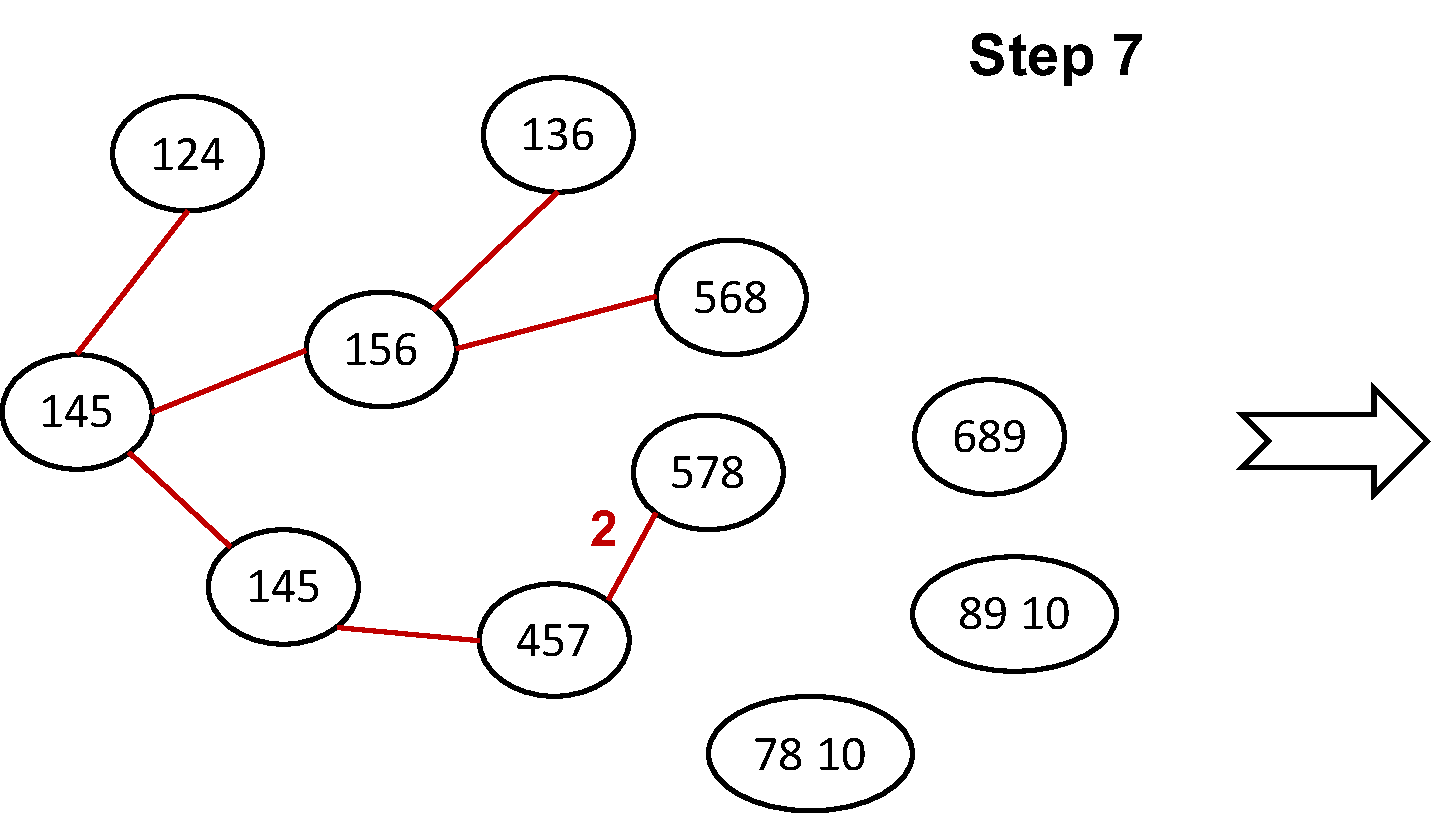
\includegraphics[width=\columnwidth]{3a9.pdf}
  \end{subfigure}
  \hspace{0.1cm}
  \begin{subfigure}[b]{0.315\textwidth}
    \centering
  	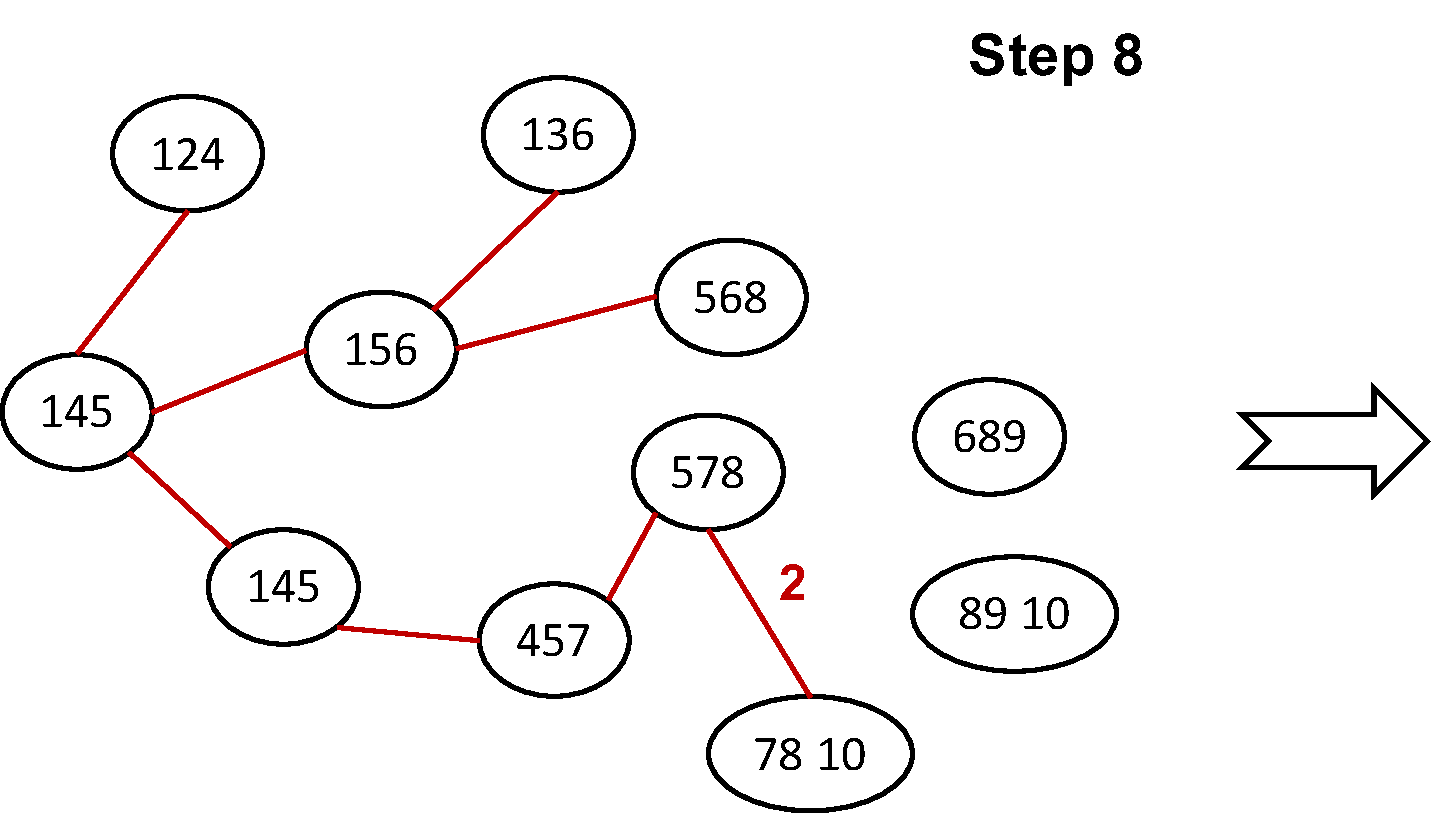
\includegraphics[width=\columnwidth]{3a10.pdf}
  \end{subfigure}
  \hspace{0.1cm}
    \begin{subfigure}[b]{0.315\textwidth}
  	\centering
  	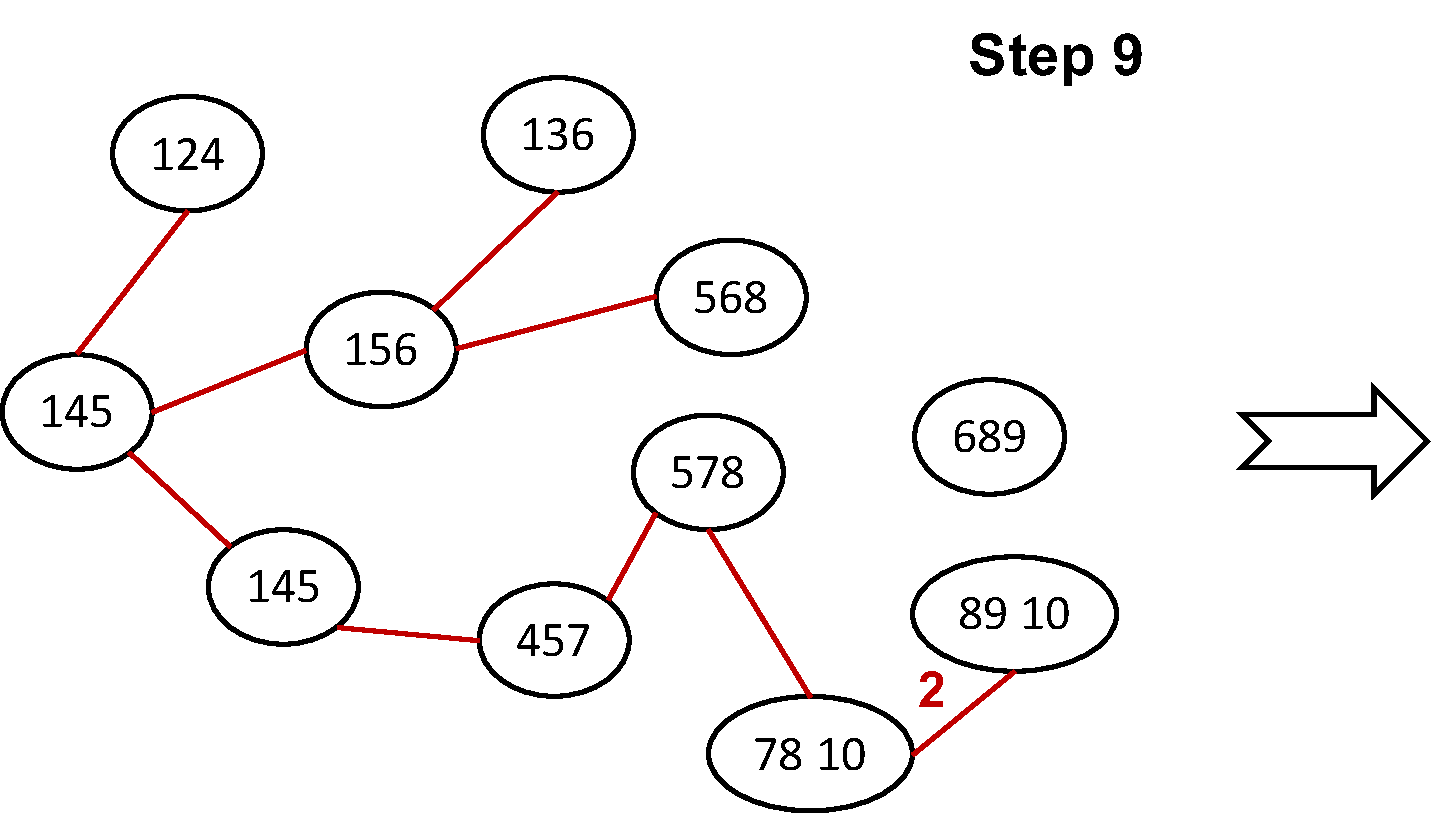
\includegraphics[width=\columnwidth]{3a11.pdf}
  \end{subfigure}
  \hspace{0.1cm}
    \begin{subfigure}[b]{0.27\textwidth}
  	\centering
  	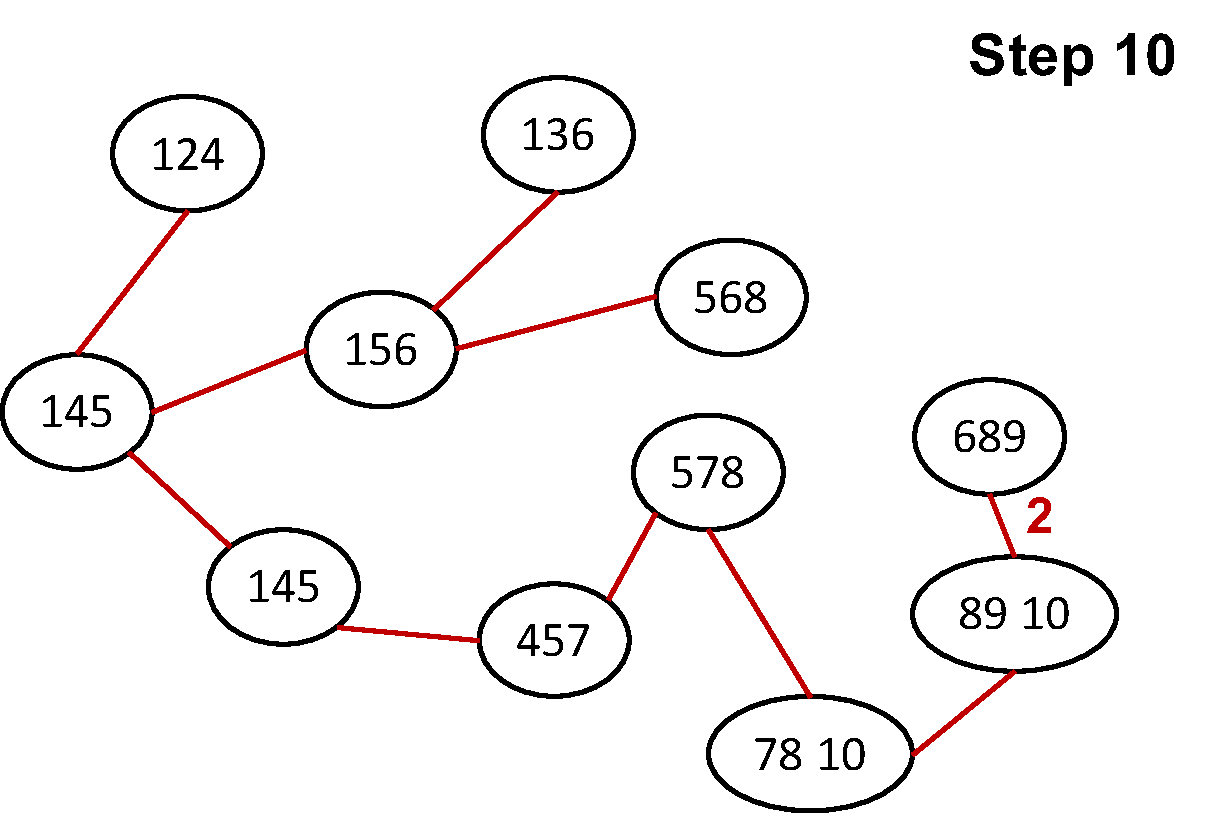
\includegraphics[width=\columnwidth]{3a12.pdf}
  \end{subfigure}
\end{figure}
\pagebreak

Since the original graph is already chordal, triangulating graph (b) gives:
\begin{figure}[h]
  \centering
  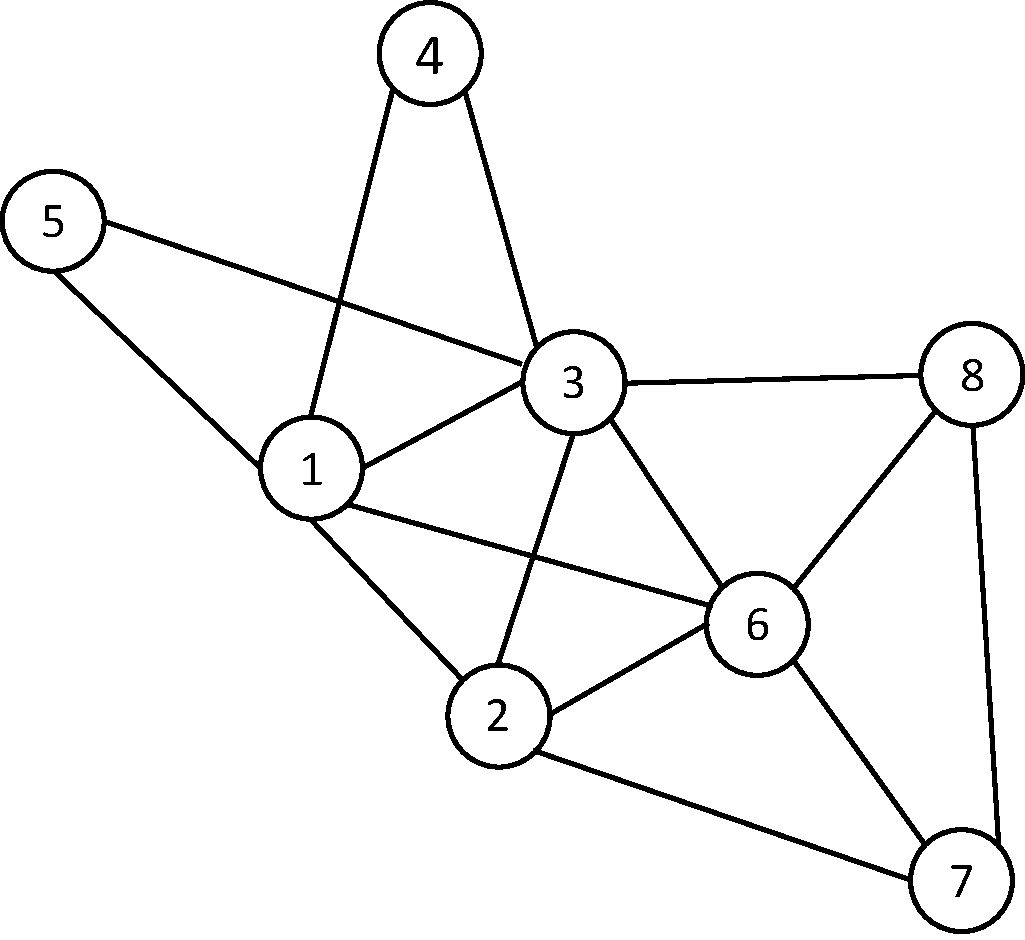
\includegraphics[width=0.25\columnwidth]{3b0.pdf}
    \vspace{-0.1cm}
\end{figure}

Applying greedy algorithm to construct the junction tree, with edge weights at each step
\begin{figure}[h]
  \centering
  \begin{subfigure}[b]{0.315\textwidth}
  	\centering
  	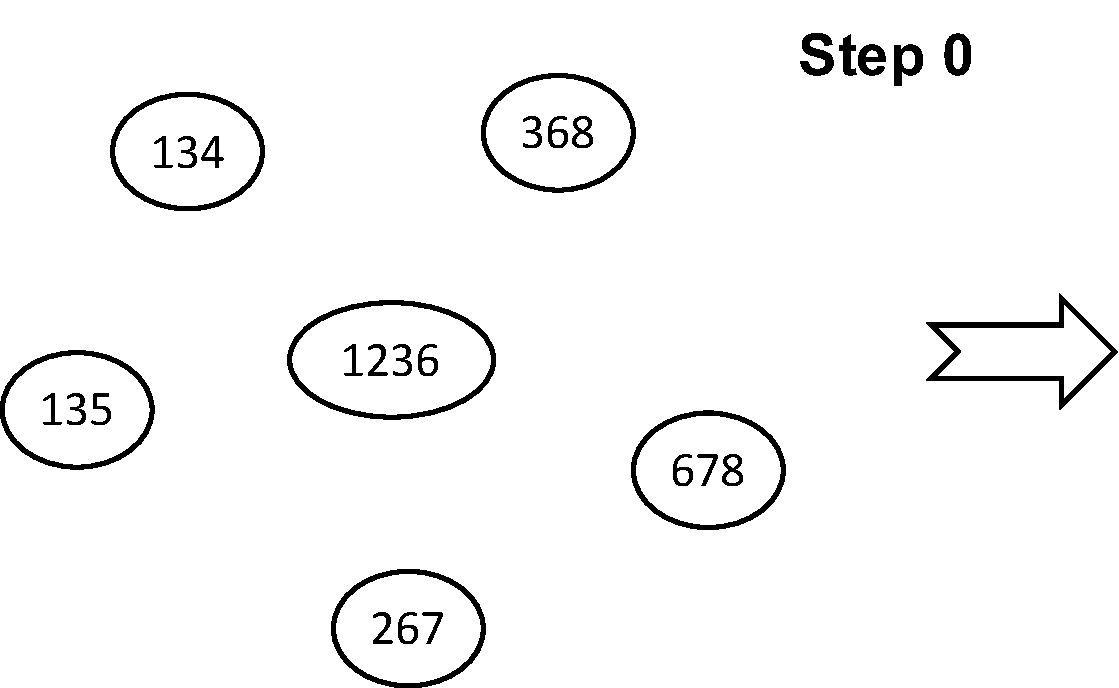
\includegraphics[width=\columnwidth]{3b1.pdf}
  \end{subfigure}
  \hspace{0.1cm}
  \begin{subfigure}[b]{0.315\textwidth}
    \centering
  	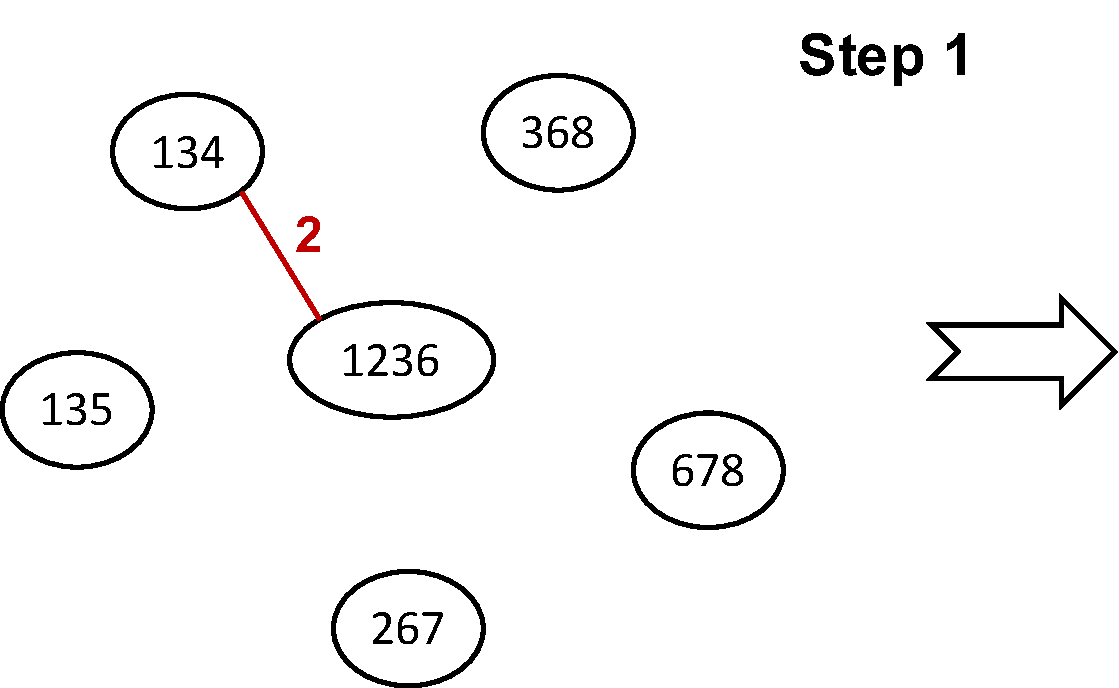
\includegraphics[width=\columnwidth]{3b2.pdf}
  \end{subfigure}
  \hspace{0.1cm}
  \begin{subfigure}[b]{0.315\textwidth}
    \centering
  	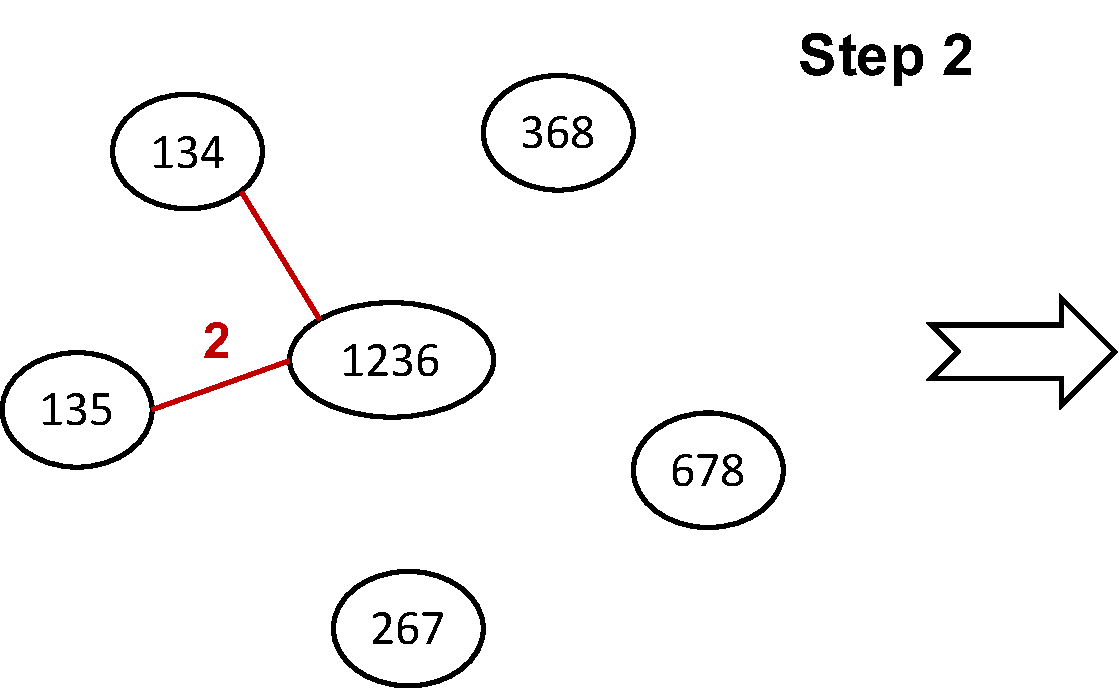
\includegraphics[width=\columnwidth]{3b3.pdf}
  \end{subfigure}
  \hspace{0.1cm}
    \begin{subfigure}[b]{0.315\textwidth}
  	\centering
  	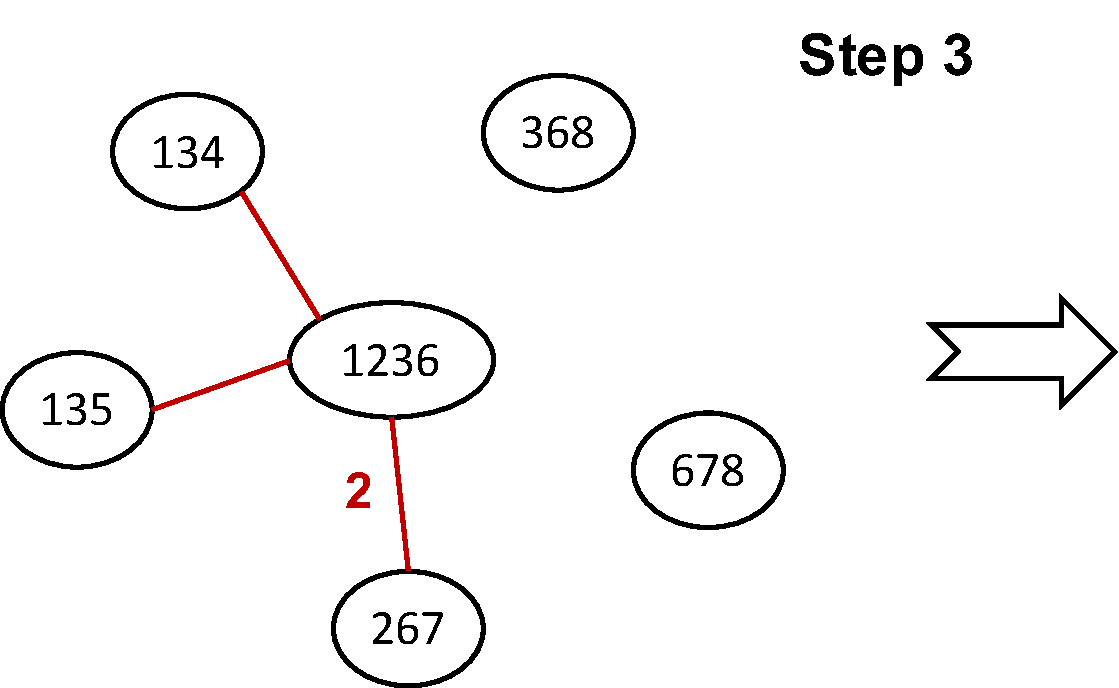
\includegraphics[width=\columnwidth]{3b4.pdf}
  \end{subfigure}
  \hspace{0.1cm}
  \begin{subfigure}[b]{0.315\textwidth}
    \centering
  	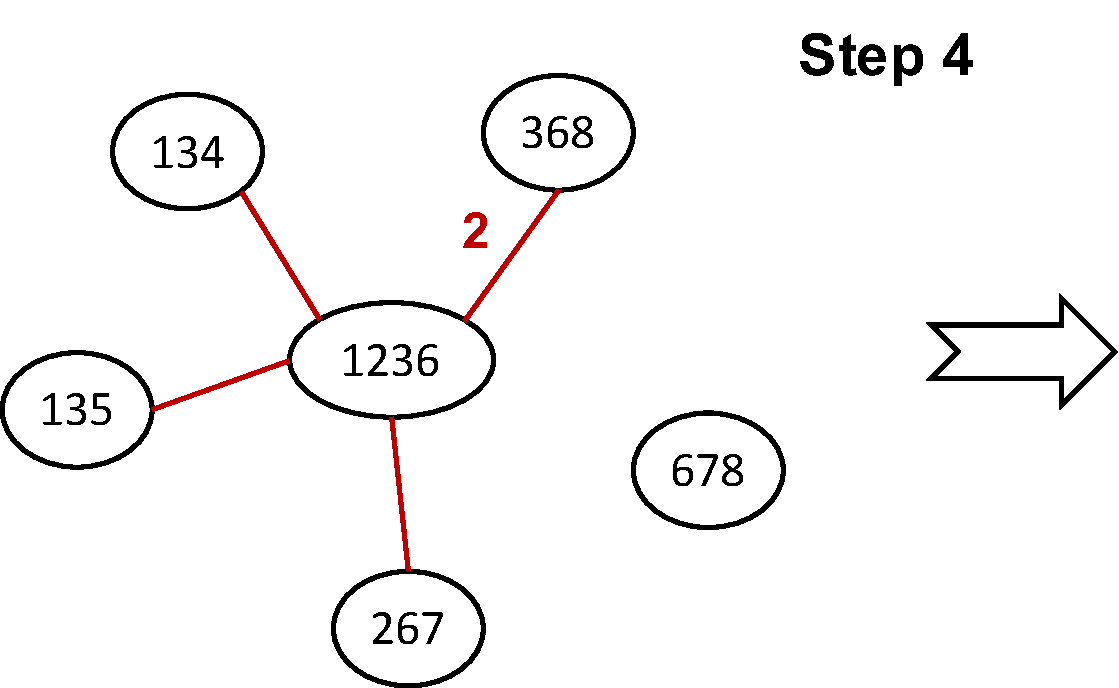
\includegraphics[width=\columnwidth]{3b5.pdf}
  \end{subfigure}
  \hspace{0.1cm}
  \begin{subfigure}[b]{0.28\textwidth}
    \centering
  	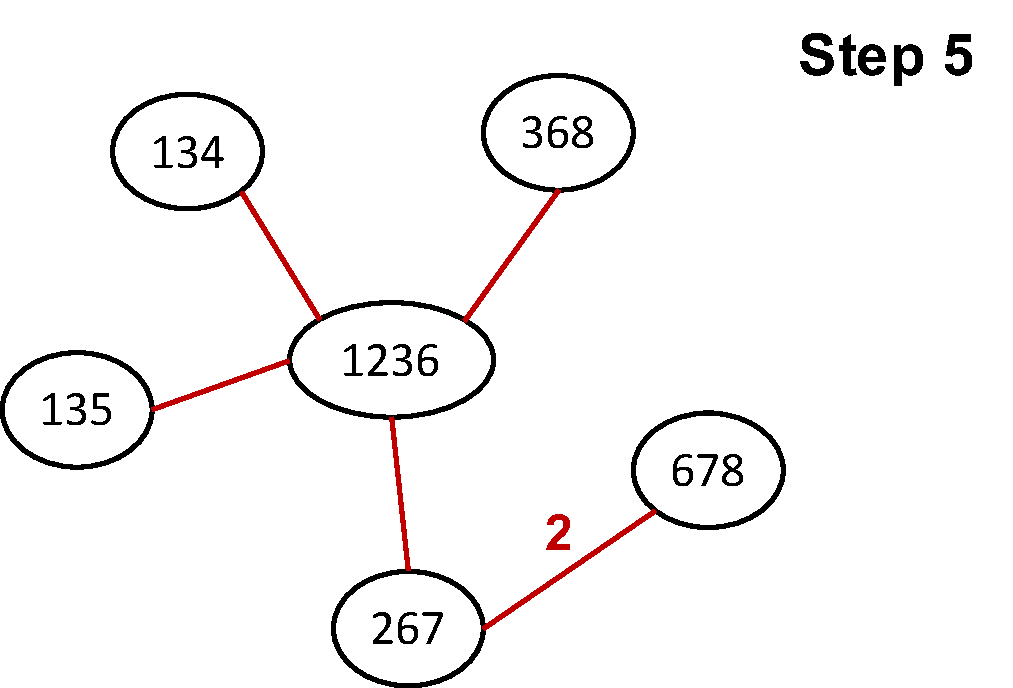
\includegraphics[width=\columnwidth]{3b6.pdf}
  \end{subfigure}
\end{figure}
\pagebreak

\pagebreak
%%%%%%%%%%%%%%%%%%%%%%%%%%%%%%%%%%%%%%%%%%%%%%%%%%%%%%%%%%%%%%%%%%%%%%%% 
\section*{Problem 4.5}
%
(a) At each loopy BP step, the message follows
\begin{align*}
	m_{j\to i}(x_i) = \sum_{x_j}\exp(\beta x_i x_j)\prod_{k\in \partial j \backslash i} m_{k\to j}(x_j),
\end{align*}
where $\partial j$ denotes the four neighboring nodes of $j$.
\\

\noindent
(b) Assume the message is invariant under translation, we have
\begin{align*}
	m(1) &= \exp(\beta)m(1)^3 + \exp(-\beta)m(-1)^3\\
	m(-1) &= \exp(-\beta)m(1)^3 + \exp(\beta)m(-1)^3.
\end{align*}
%

Therefore, 
\begin{align}
	m(x) = \exp(\beta)m(x)^3 + \exp(-\beta)m(-x)^3. \label{eq:5b}
\end{align}
\\

\noindent
(c) Massaging terms in $h$, we have
\begin{align*}
	m(1) &= \exp(2\beta h)m(-1)\\
	m(-1) &= \exp(-2\beta h)m(1).
\end{align*}
%

Since $Z = m(1) + m(-1)$,
\begin{align*}
	Z &= m(1) + \exp(-2\beta h)m(1)\\
	Z &= \exp(2\beta h)m(-1) + m(-1).
\end{align*}
%

Thus,
\begin{align}
	m(x) = \frac{Z}{1 + \exp(-2\beta h x)}. \label{eq:5c}
\end{align}
%

Now we plug in results from (b) for $m(1) / m(-1)$, we have
\begin{align*}
	\exp(2\beta h) = \frac{m(1)}{m(-1)} &=
	\frac{\exp(\beta)m(1)^3 + \exp(-\beta)m(-1)^3}{\exp(-\beta)m(1)^3 + \exp(\beta)m(-1)^3} \\
	&=\frac{\frac{\exp(\beta)Z^3}{\big[1 + \exp(-2\beta h)\big]^3} +
	  \frac{\exp(-\beta)Z^3}{\big[1 + \exp(2\beta h)\big]^3}}
	  {\frac{\exp(-\beta)Z^3}{\big[1 + \exp(-2\beta h)\big]^3} + 
	  \frac{\exp(\beta)Z^3}{\big[1 + \exp(2\beta h)\big]^3}}\\
	&=\frac{\frac{\exp(\beta)\exp(6\beta h)}{\big[\exp(2\beta h) + 1\big]^3} +
	  \frac{\exp(-\beta)}{\big[1 + \exp(2\beta h)\big]^3}}
	  {\frac{\exp(-\beta)\exp(6\beta h)}{\big[\exp(2\beta h) + 1\big]^3} + 
	  \frac{\exp(\beta)}{\big[1 + \exp(2\beta h)\big]^3}}\\
	&=\frac{\exp(\beta)\exp(3\beta h) +
	        \exp(-\beta)\exp(-3\beta h)}
	       {\exp(-\beta)\exp(3\beta h) +
	        \exp(\beta)\exp(-3\beta h)}.
\end{align*}
%

Finally,
\begin{align*}
	\tanh(\beta h) &= \frac{\exp(2\beta h) - 1}{ \exp(2\beta h) + 1} \\
	&= \frac{\frac{\exp(\beta)\exp(3\beta h) +
	        \exp(-\beta)\exp(-3\beta h)}
	       {\exp(-\beta)\exp(3\beta h) +
	        \exp(\beta)\exp(-3\beta h)} - 1}
	        {\frac{\exp(\beta)\exp(3\beta h) +
	        \exp(-\beta)\exp(-3\beta h)}
	       {\exp(-\beta)\exp(3\beta h) +
	        \exp(\beta)\exp(-3\beta h)} + 1} \\
    &= \frac{\exp(\beta)\exp(3\beta h) + \exp(-\beta)\exp(-3\beta h) -
             {\exp(-\beta)\exp(3\beta h) - \exp(\beta)\exp(-3\beta h)}}
            {\exp(\beta)\exp(3\beta h) + \exp(-\beta)\exp(-3\beta h) +
             {\exp(-\beta)\exp(3\beta h) + \exp(\beta)\exp(-3\beta h)}} \\
    &= \frac{\big[\exp(\beta) - \exp(-\beta)\big]
             \big[\exp(3\beta h) - \exp(-3\beta h)\big]}
            {\big[\exp(\beta) + \exp(-\beta)\big]
             \big[\exp(3\beta h) + \exp(-3\beta h)\big]}\\
    &= \tanh(\beta) \tanh(3\beta h).
\end{align*}\qeds
\\

\noindent
(d) Since $m(x) = Z/\big(1 + \exp(-2\beta h x)\big)$, we only need to determine the value
of $\beta h$ to find the fixed message. We denote $k = \beta h$. Notice from (c) that
\begin{align*}
	\frac{\tanh(k)}{\tanh(3k)} = \frac{\tanh(\beta h)}{\tanh(3\beta h)} = \tanh(\beta).
\end{align*}
%
\begin{figure}[h]
  \centering
  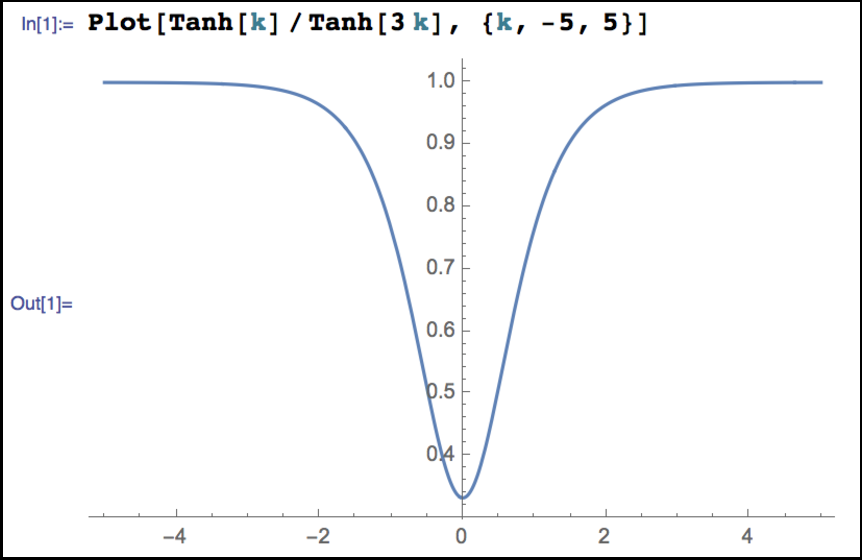
\includegraphics[width=0.4\columnwidth]{5d.pdf}
    \vspace{-0.1cm}
  \caption{$\tanh(k)/\tanh(3k)$, plotted over $k\in(-5,5)$. The intersection with y-axis is at $1/3$.}
  \label{f:5d}
\end{figure}
%

To find the solution fo $k$ is equivalent to find the intersection of $\tanh(k)/\tanh(3)$ and $\tanh(\beta)$.
We first note that $\tanh(0) = 0$, $\tanh'(k) = \text{sech}(k)$ and $\tanh'(3k) = 3\text{sech}(k)$,
applying L'Hospital's Rule,
\begin{align*}
	\lim_{k\to 0} \frac{\tanh(k)}{\tanh(3k)} = \lim_{k\to 0} \frac{\tanh'(k)}{\tanh'(3k)} = \lim_{k\to 0} \frac{\text{sech}(k)}{3\text{sech}(k)} = \frac{1}{3}.
\end{align*}

Second, note that $\tanh(k)/\tanh(3k)$ is symmetric, i.e., 
\begin{align*}
	\frac{\tanh(-k)}{\tanh(-3k)} = \frac{-\tanh(k)}{-\tanh(3k)} = \frac{\tanh(k)}{\tanh(3k)}.
\end{align*}

Lastly, $\tanh(k)/\tanh(3k)$ increases monotonically for $k>0$ (and decreases monotonically for $k<0$).
This is  because we can write
\begin{align*}
	\frac{\tanh(k)}{\tanh(3k)} &= \frac{\exp(k) - \exp(-k)}{\exp(k) + \exp(-k)}
	\times\frac{\exp(3k) + \exp(-3k)}{\exp(3k) - \exp(-3k)}\\
	&=\frac{\exp(k) - \exp(-k)}{\exp(k) + \exp(-k)}\times
	\frac{\exp(k) + \exp(-5k)}{\exp(k) - \exp(-5k)}.
\end{align*}
Here, as $k>0$ increases, $\exp(-k)$ gets increasingly smaller; and $\exp(-k)$ always overwhelms $\exp(-5k)$.
As a result, $\tanh(k)/\tanh(3k)$ monotonically increases for $k>0$. The upper bound for this expression is
\begin{align*}
	\lim_{k\to\infty}\frac{\tanh(k)}{\tanh(3k)} &= 
	\lim_{k\to\infty}\frac{\exp(k) - \exp(-k)}{\exp(k) + \exp(-k)}
	\times\lim_{k\to\infty}\frac{\exp(3k) + \exp(-3k)}{\exp(3k) - \exp(-3k)}\\
	&= \lim_{k\to\infty}\frac{1 - \exp(-2k)}{1 + \exp(-2k)}
	\times\lim_{k\to\infty}\frac{1 + \exp(-6k)}{1 - \exp(-6k)}\\
	&= 1.
\end{align*}

Figure~\ref{f:5d} visualizes $\tanh(k)/\tanh(3k)$. Therefore, when $\tanh(\beta) > 1/3$ (notice 
$\lim_{\beta\to\pm\infty}\tanh(\beta)=1$), $\tanh(k)/\tanh(3k) = \tanh(\beta)$ will have two
symmetric solutions. Moreover, since $m(x) = 0$ is always a solution (not expressed by Equation~\eqref{eq:5c}),
the LBP has three distinct fixed points. \qeds
\\

\noindent
(e) For ferromagnetic Ising model, we assume temperature $\beta >0$. The convergence of LBP depends on the 
initialization of $m(1)$ and $m(-1)$. Specifically,
\begin{enumerate}
	\item Initializing $m(1) = m(-1)$, i.e., $h=\frac{1}{2\beta}\log \frac{m(1)}{m(-1)} = 0$, LBP converges to
	the fixed point at 0 for all $\beta > 0$. We can check this in the update equation
	$m(1) = m(-1) = [\exp(\beta) + \exp(-\beta)]m(1)^3$
	(assume that we perform normalization after each update step).
	\item With initialization $m(1) > m(-1)$, i.e., $h=\frac{1}{2\beta}\log \frac{m(1)}{m(-1)} > 0$, and
	$\tanh(\beta) > 1/3$ from (c), LBP 
	converges to the positive fixed point. This can be shown by considering
	\begin{align*}
		\left[\frac{m(1)}{m(-1)}\right]_t &= 
		\frac{\exp(\beta)m_t(1)^3 + \exp(-\beta)m_t(-1)^3}{\exp(-\beta)m_t(1)^3 + \exp(\beta)m_t(-1)^3}\\
		&=\frac{\exp(\beta)\big[m(1)/m(-1)\big]_t^3 +
		\exp(-\beta)}{\exp(-\beta)\big[m(1)/m(-1)\big]_t^3 + \exp(\beta)}.
	\end{align*}
	Let $\mu_t = \big[m(1)/m(-1)\big]_t$ for each iteration step $t$, we have
	\begin{align*}
		\mu_{t+1} = \frac{\exp(2\beta)\mu_t^3 + 1}{\mu_t^3 + \exp(2\beta)}.
	\end{align*}
	Here, the iterative update for $\mu_t$ is a monotonically increasing function and $\mu$ is upper bounded
	by $\exp(2\beta)$. Therefore, the iterative update must converge. From (c) we know $\tanh(\beta) > 1/3$ 
	yields a positive fixed point that the iterative update will converge to.
	\item Similarly, with initialization $m(1) < m(-1)$, 
	i.e., $h=\frac{1}{2\beta}\log \frac{m(1)}{m(-1)} < 0$, and
	$\tanh(\beta) > 1/3$ from (c), LBP 
	converges to the negative fixed point. The argument follows the previous case.
\end{enumerate}

\noindent
(f) The fixed point evolves from 0 to the positive or negative fixed point (depending on the initialization of $m(1)/m(-1)$). The tipping point for transition from neutral to polarized is when $\tanh(\beta_c) > 1/3$. The approximate value of the critical temperature is given by
\begin{align*}
	\beta_c = \tanh^{-1}\left(\frac{1}{3}\right)\approx0.3466.
\end{align*}


\end{document}